% Copyright 2019 by Junan Lin <junan_lin@hotmail.com>
% This file may be distributed and/or modified under the MIT license
% Reference: https://ramblingacademic.com/2015/12/08/how-to-quickly-overhaul-beamer-colors/
\documentclass[xcolor=dvipsnames]{beamer}

\mode<presentation>{\setbeamercovered{invisible}
\usetheme{Madrid}
}

% Customize for Waterloo theme (gold and black)
\definecolor{UWgold}{RGB}{254,209,66} % Waterloo gold
\definecolor{darkgrey}{RGB}{169,169,169} 
\usepackage[font=tiny,labelfont=bf,margin=25pt]{caption} % changes settings for caption

\usepackage{bin/._math}
\usepackage{commath}
\usepackage{physics}
\usepackage{amsmath}
\usepackage{amssymb}

% BIB SETTINGS
\usepackage[
    backend=biber,
    giveninits=true,
    maxnames=30,
    maxcitenames=20,
    uniquename=init,
    url=true,
    style=verbose,
]{biblatex}
\addbibresource{ref.bib}
%\setlength\bibitemsep{0.3cm} % space between entries in the reference list
\renewcommand{\bibfont}{\normalfont\scriptsize}
\setbeamerfont{footnote}{size=\tiny}
\renewcommand{\cite}[1]{\footnote<.->[frame]{\fullcite{#1}}}
% \setlength{\TPHorizModule}{\paperwidth}
% \setlength{\TPVertModule}{\paperheight}
%\nocite{*} % print entire bibliography
\bibliographystyle{ieeetr}

\setbeamercolor{palette primary}{bg=black,fg=UWgold}
\setbeamercolor{palette secondary}{bg=white,fg=black}
\setbeamercolor{palette tertiary}{bg=UWgold,fg=white}
\setbeamercolor{palette quaternary}{bg=Black,fg=white}
\setbeamercolor{structure}{fg=darkgrey} % itemize, enumerate, etc
\setbeamercolor{section in toc}{fg=black} % TOC sections
\setbeamercolor{section in head/foot}{bg=UWgold,fg=white}


\usepackage{graphicx} % Allows including images

%Includes TOC at the begging of each section
% \AtBeginSection[]
% {
%   \begin{frame}
%     \frametitle{Contents}
%     \tableofcontents[currentsection]
%   \end{frame}
% }

\title[PHYS 437A]{\large Examples of Dynamical Reduction Using Symmetry\\for Simple Mechanical Systems with Virtual Holonomic Constraints}
\author{Emrys Halbertsma}
\institute[UWaterloo]
{    
    Department of Physics \& Astronomy,\\
        University of Waterloo\\
        \medskip
        Supervised by\\\vspace{0.55mm}
    {\normalsize Dr. Christopher Nielsen}\\\medskip
        Department of Electrical \& Computer Engineering,\\
        University of Waterloo
% University of Waterloo, Waterloo, ON, Canada\\
% \medskip
% \textit{egthalbe@uwaterloo.ca}
}
\date{\tiny \today}

\titlegraphic{\makebox[\linewidth]{
\includegraphics[height=.15\textheight]{assets/UniversityOfWaterloo_logo_horiz_rgb.png}}}
%\logo{
\includegraphics[width=.2\paperwidth]{assets/UniversityOfWaterloo_logo_horiz_rgb}}

\begin{document}
	
\begin{frame}
	\titlepage % Print the title page as the first slide
\end{frame}

\begin{frame}
	\frametitle{Agenda}
	\tableofcontents
\end{frame}

\section{Introduction}
\begin{frame}{Underactuated Robotics}
\begin{figure}
    \centering
    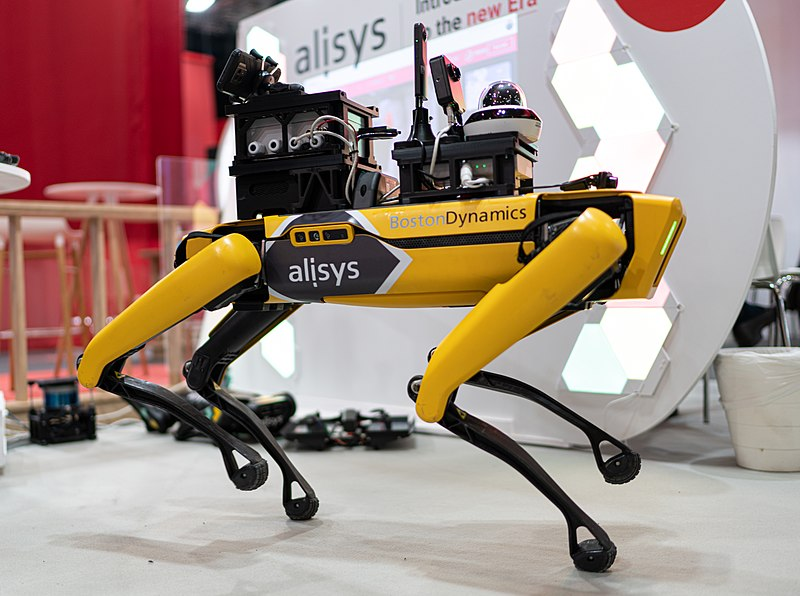
\includegraphics[width=.25\textwidth]{assets/bostondyn.png}
    \caption{Modern underactuated robot\cite{bostondyn}}
    \label{fig:bostondyn}
\end{figure}
	\begin{itemize}
 \item Modern robotic systems are \textbf{underactuated}: there are more degrees of freedom than actuators \cite{underactuated}. 
\item Robots with $\geq 2$ degrees of underactuation may have complex dynamics
	\end{itemize}
\end{frame}

\begin{frame}{Motivation}
Robotics engineers need mathematical methods to control underactuated robots that are:
\begin{itemize}
    \item \textbf{Fast}: the robot can respond in real time
    \item \textbf{Reliable}: the robots follows the planned trajectory
    \item \textbf{Stable}: the robot can deal with disturbances
    \item \textbf{Efficient}: minimize computation for small embedded computers
\end{itemize}
\begin{figure}
    \centering
    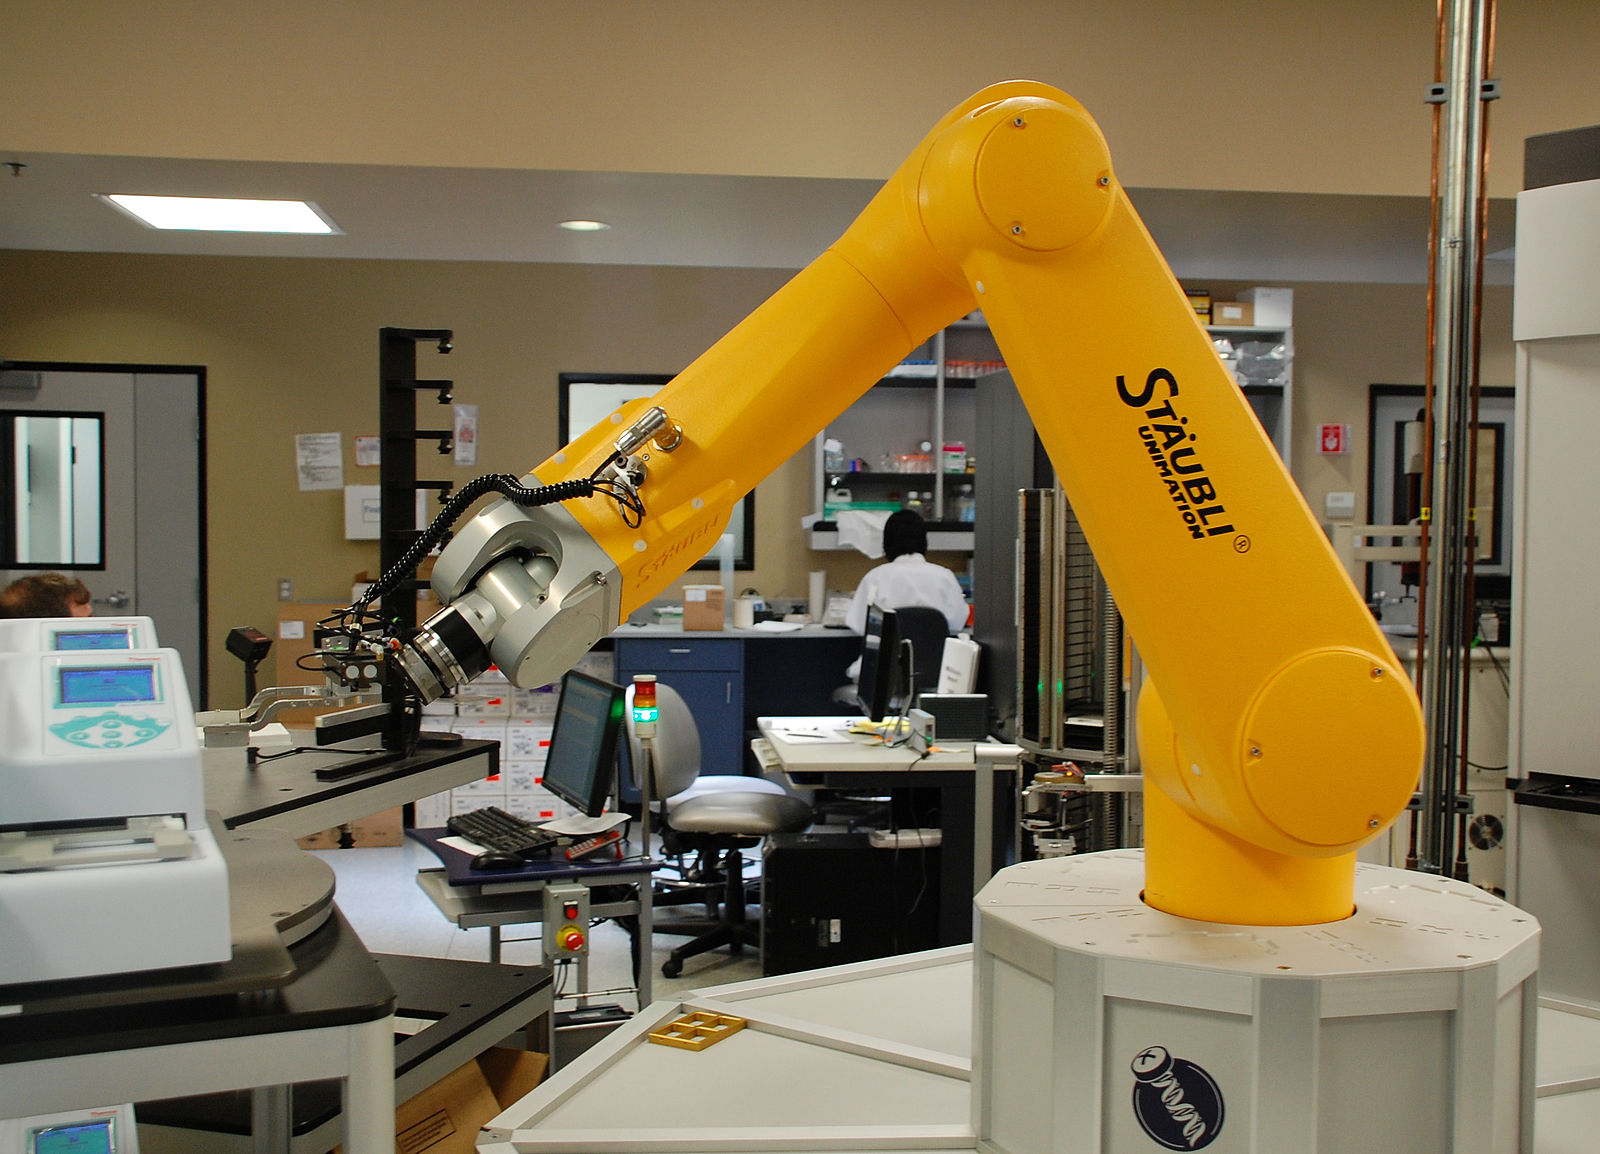
\includegraphics[width=0.25\textwidth]{assets/robotarmfactory.jpg}
    \caption{Robotic arm used in industrial applications\cite{robotarmfactory}}
    \label{fig:robotarmfactory}
\end{figure}
\end{frame}

\section{Problem Definition}
\begin{frame}{Problem Definition}
This project considers a particular class of systems with the following traits:
\begin{itemize}
    \item \textbf{Simple}\footnote{``Simple Mechanical Control System", as defined in Bullo, Lewis \textsl{Geometric Control of Mechanical Systems}}: mechanical system such as a pendulum
    \item \textbf{Underactuated}: $\mathrm{coordinates}-\mathrm{actuators}\geq 2$
    \item \textbf{Symmetric}: 1 or more symmetries in the Lagrangian
    \item \textbf{Constrained}: subject to Virtual Holonomic Constraints
\end{itemize}
\end{frame}

\begin{frame}{Virtual Holonomic Constraints}
A \textbf{holonomic constraint} is a precise restriction on the position variables of a mechanical system\cite{marsden2013introduction}.

It can always be expressed as a homogeneous function:
\begin{align}
    f(x_1,x_2,\ldots)=0 && f(x,y):=x^2+y^2-L^2=0
\end{align}
\begin{figure}
    \centering
    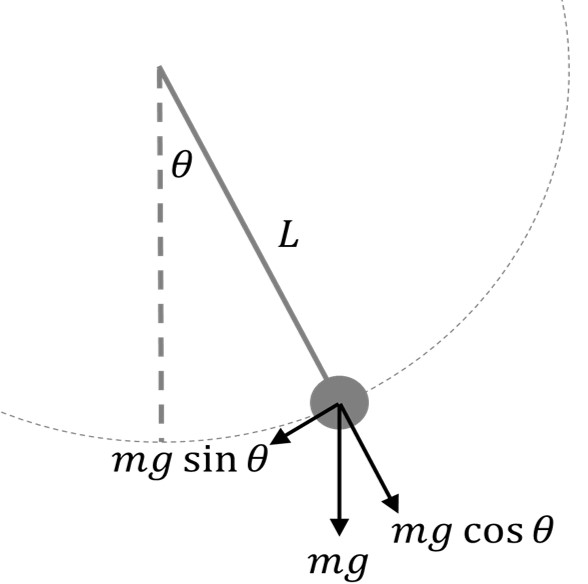
\includegraphics[width=0.3\textwidth]{assets/pendulumswing.jpg}
    \caption{The pendulum's length $L$ is holonomically constrained\cite{pendulum}}
    \label{fig:pendulum}
\end{figure}
\end{frame}

\begin{frame}{Virtual Holonomic Constraints}
A \textbf{Virtual Holonomic Constraint} is similar, however, the constraint is applied through \textbf{feedback control}\cite{maggiore2012virtual}.
\begin{figure}
    \centering
    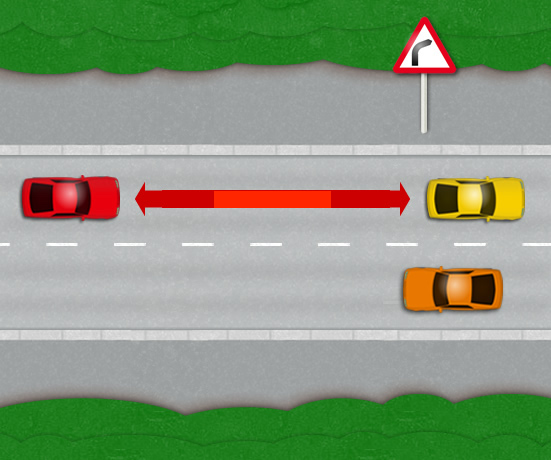
\includegraphics[width=0.2\textwidth]{assets/2-second-rule-300x250.jpg}
    \caption{Vehicles on a highway\cite{cars}}
    \label{fig:cars}
\end{figure}
\begin{itemize}
    \item \textbf{Holonomic}: the cars maintain a fixed distance because they are mechanically linked with a chain
    \item \textbf{Virtual Holonomic}: the vehicles maintain a fixed distance because Red's adaptive cruise control actively tunes the throttle to always match Yellow's speed
\end{itemize}
\end{frame}

\section{Methodology}
\begin{frame}{Methodology}
A simple, underactuated, symmetric system subject to VHCs 
can be dynamically reduced to two independent ``vertical" and ``horizontal" vector fields, resulting in simpler control dynamics\cite{mccarthy}.
\\\medskip
We compute and simulate the reduced dynamics of two such systems:
\begin{itemize}
    \item Offset Robotic Arm
    \item Spherical Pendulum
\end{itemize}
\end{frame}

\section{Results}
\begin{frame}{Offset Robotic Arm}
\begin{figure}
    \centering
    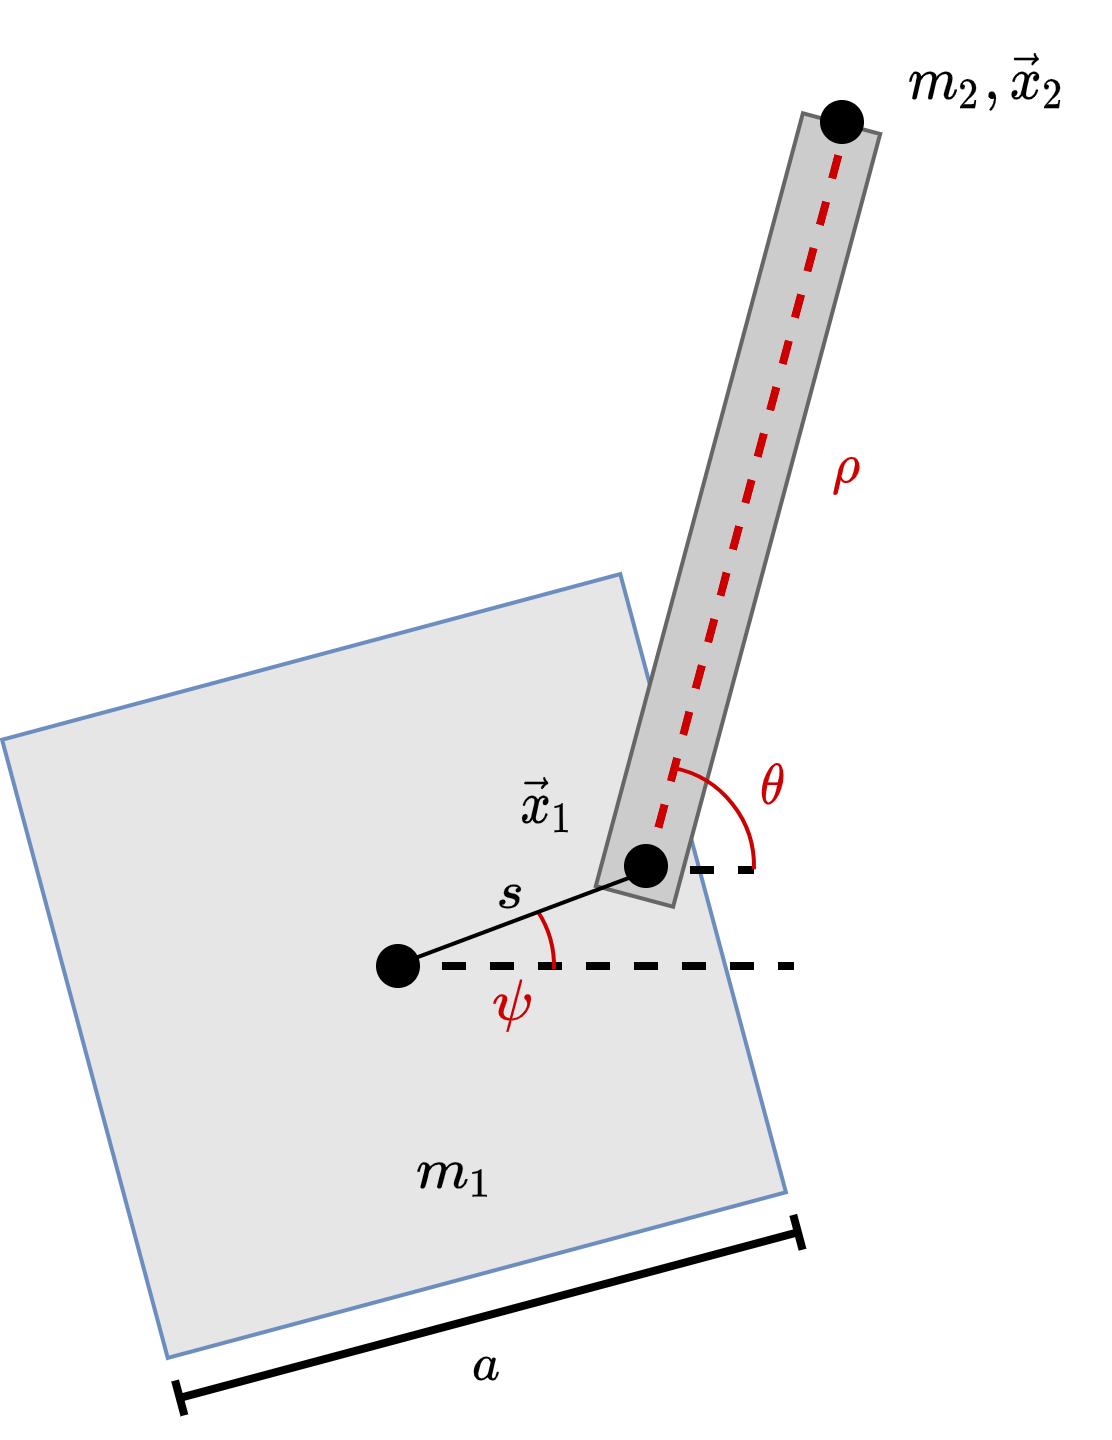
\includegraphics[width=0.35\textwidth]{assets/robot-arm.png}
    \caption{Offset robotic arm schematic diagram}
    \label{fig:robarm}
\end{figure}
	\begin{itemize}
		\item Degrees of freedom: rod rotates in $\theta$, block rotates in $\psi$
		\item Actuators: block actuates in $\psi$
	\end{itemize}
\end{frame}

\begin{frame}{Offset Robotic Arm}
After deriving the Lagrangian of the system, it was shown that the system is symmetric in $\theta-\psi$. Based on the symmetry, the chosen holonomic constraint is
\begin{align}
    h(\theta,\psi):=\theta-\psi=0.
\end{align}
Under this constraint, the configuration manifold is
\begin{align}
     \mathcal{C}=\cbr{\theta,\phi\in Q:\theta=\psi}
\end{align}
This is parametrized and solved to give the constrained dynamics: 1 second-order DE. 
\end{frame}

\begin{frame}{Offset Robotic Arm}
The constrained dynamics are then reduced further.
\begin{itemize}
    \item Use McCarthy's method to compute the ``vertical" vector field (from the symmetry and the VHC)
    \begin{align}
        V:=\pdv{\Phi}{g}
    \end{align}
    \item Choose a ``horizontal" vector field based on the tangent space of the constraint space.
    \begin{align}
        H:=\nabla_q h(q)
    \end{align}
\end{itemize}
\textbf{Result}: the constrained dynamics can be expressed simply using the $V$ and $H$ vectors.
\end{frame}

\begin{frame}{Offset Robotic Arm}
\begin{figure}[h]
    \centering
    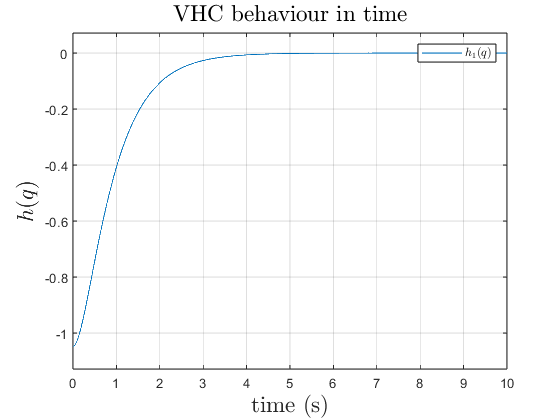
\includegraphics[width=0.48\textheight]{assets/rao1.png}
    %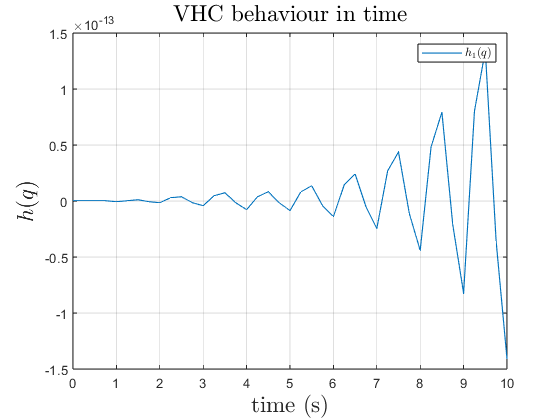
\includegraphics[width=0.48\textheight]{assets/rao2.png}
    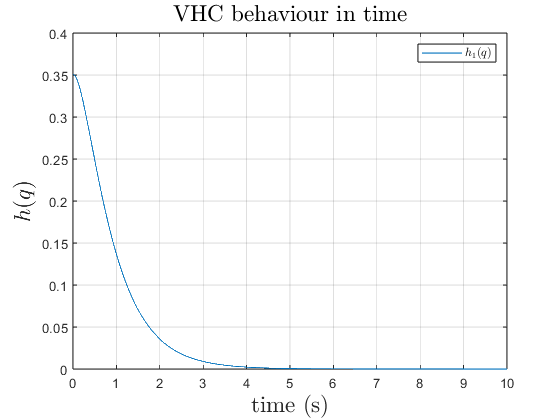
\includegraphics[width=0.48\textheight]{assets/rao3.png}
    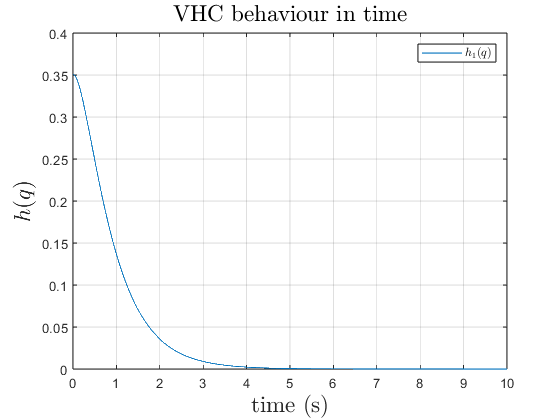
\includegraphics[width=0.48\textheight]{assets/rao4.png}
    \caption{Plot showing convergence of the VHCs (control error) towards zero on the Offset Robotic Arm model. Here, the constraint is defined using the equivalent $h:=\arg\cbr{\exp(i[\theta-\psi])}$.}
    \label{fig:graph-robotarm}
\end{figure}
\end{frame}

\begin{frame}{Spherical Pendulum}
\begin{figure}
    \centering
    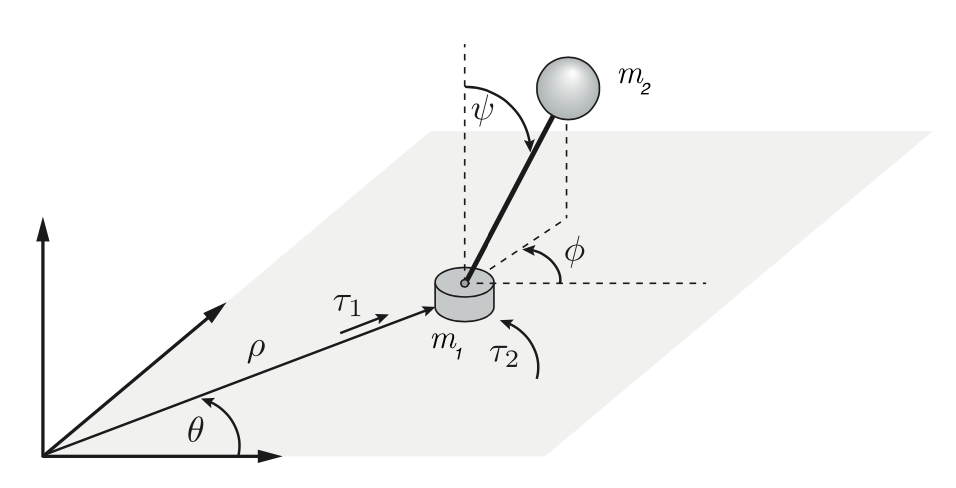
\includegraphics[width=0.66\textwidth]{assets/spherical-pen.png}
    \caption{Spherical pendulum schematic diagram\cite{mccarthy}}
    \label{fig:spendulum}
\end{figure}
	\begin{itemize}
		\item Degrees of freedom: $\rho,\theta,\phi,\psi$
		\item Actuators: radial $\tau_1$, tangential $\tau_2$
	\end{itemize}
\end{frame}

\begin{frame}{Offset Robotic Arm}
The configuration manifold is $Q=\mathbb{R}_{>0}\cross\mathbb{S}^1\cross\mathbb{S}^2$.

After deriving the Lagrangian of the system, it was shown that the system is symmetric in $\theta-\phi$. Based on the symmetry, the chosen holonomic constraint is
\begin{align}
    h(\rho,\theta,\phi,\psi):=\pmqty{\theta-\phi\\\psi-\frac{\pi}{4}\tanh \rho}=\pmqty{0\\0}.
\end{align}
Under this constraint, the constrained configuration manifold is
\begin{align}
    \mathcal{C}=\cbr{\rho,\theta,\phi\psi\in Q:\theta=\phi,psi=\frac{\pi}{4}\tanh \rho}\subseteq Q.
\end{align}
A similar process as above is taken to compute the constrained and reduced dynamics.
\end{frame}

\begin{frame}{Spherical Pendulum}
    \begin{figure}[h]
    \centering
    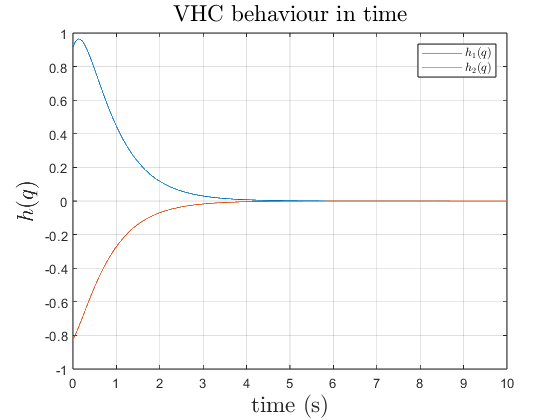
\includegraphics[width=0.48\textheight]{assets/sp1.png}
    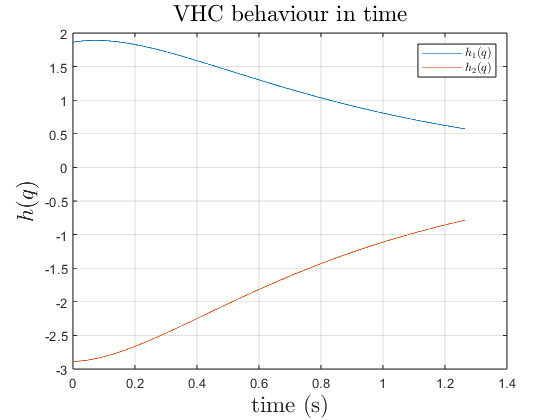
\includegraphics[width=0.48\textheight]{assets/sp2.png}
    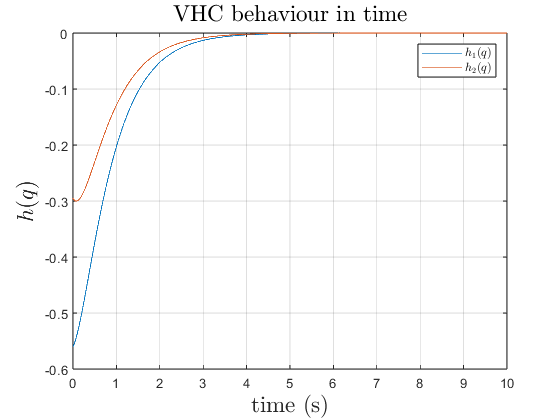
\includegraphics[width=0.48\textheight]{assets/sp3.png}
    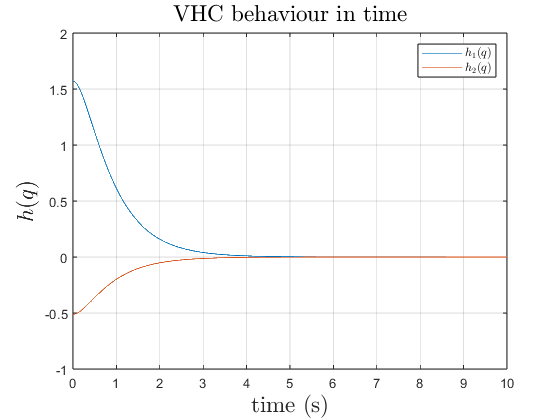
\includegraphics[width=0.48\textheight]{assets/sp4.png}
        \caption{Plot showing convergence of the VHCs (control error) towards zero on the Spherical Pendulum model. Here, the constraint is defined $h_1:=\theta-\phi, h_2=\psi-\frac{\pi}{4}\tanh \rho.$}
    \label{fig:graph-pendulum}
\end{figure}
\end{frame}

\section{Conclusion}
\begin{frame}{Conclusion}
% A mechanical system can be made to appear holonomically constrained by actively enforcing a constraint through control. These so-called Virtual Holonomic Constraints (VHCs) have useful applications in robotics, such as maintaining set distances between agents or synchronizing the motions of joints. 
% A mechanical system subject to such VHCs, the system is driven towards a submanifold of its configuration manifold, but its dynamics are not necessarily Euler-Lagrange on the constraint manifold.
% This project considers some examples of simple, 2\tss{nd}-degree underactuated mechanical systems with 1 degree of symmetry. Using Matlab, the mechanical systems are modelled and analyzed. The tangent spaces of their constraint manifolds are computed, along with the system's constrained dynamics, and then decomposed into an Ehresmann-like connection of Vertical and Horizontal Vector fields. The dynamical reduction technique can prove useful in simplifying the dynamics of robotic applications requiring the enforcement of a Virtual Holonomic Constraints.	
 \begin{itemize}
		\item Example symmetric mechanical systems were analyzed:
  \begin{itemize}
      \item Derived symmetry and Euler-Lagrange dynamics
      \item Selected appropriate VHCs according to the symmetry behaviour
      \item Created models in Matlab to show convergence towards the VHC conditions
      \item Computed the reduced dynamics
  \end{itemize}
            \item McCarthy's dynamical reduction technique can prove useful in simplifying the dynamics of robotic applications  subject to VHCs.
	\end{itemize}
\end{frame}

\begin{frame}{Personal Takeaways}
\begin{itemize}
    \item Underactuated robotics blends areas in math, physics, and engineering
    \item Dive into the literature to learn the conventions and state of your field
    \item Documenting on-the-go is essential
    \item Understand the purpose and audience of the project, and work towards fulfilling that purpose for your audience
\end{itemize}
\end{frame}

\section{References}
\begin{frame}[allowframebreaks,t]{\bibname}
	% the 'I' is caused by 'allowframebreaks'
	\AtNextBibliography{\footnotesize}% or in the preamble \AtBeginBibliography{\small}
	\printbibliography
\end{frame}

\end{document}
